% !TEX root = task-2-7-3.tex
% Editable task bank. Append new BankTask blocks at the end of the document.
\documentclass[12pt,a4paper]{article}
\usepackage{physics-textbook}
\usepackage{graphicx,needspace}
\usetikzlibrary{decorations.pathmorphing}
\newif\ifShowSolutions
\ifdefined\TutorEdition
  \ShowSolutionstrue
\else
  \ShowSolutionsfalse % Change to \ShowSolutionstrue to display solutions.
\fi
\newcounter{banktask}
\newsavebox{\BankTaskBox}
\newcommand{\BankTaskContent}[3]{%
  \noindent\textbf{\thebanktask.}\quad #2\par
  \ifShowSolutions
    \Needspace{50mm}% Keep the solution heading with its opening text or diagram.
    #3\par
    \ifdefined\TutorEdition
      \ifcsname TutorSource#1\endcsname
        \nopagebreak\smallskip{\small\csname TutorSource#1\endcsname\par}%
      \fi
    \fi
  \fi
}
\newcommand{\BankTask}[3]{%
  \refstepcounter{banktask}\par\medskip
  \sbox{\BankTaskBox}{\begin{minipage}{\linewidth}%
    \BankTaskContent{#1}{#2}{#3}\end{minipage}}%
  \ifdim\dimexpr\ht\BankTaskBox+\dp\BankTaskBox\relax>\dimexpr\textheight-20mm\relax
    \Needspace{35mm}\BankTaskContent{#1}{#2}{#3}%
  \else
    \Needspace{\dimexpr\ht\BankTaskBox+\dp\BankTaskBox\relax}%
    \noindent\usebox{\BankTaskBox}\par
  \fi
  \medskip
}
\begin{document}
\BookSubsection{2.7.3}{Насыщенный пар и динамическое равновесие}


% Source sdamgia-3326: https://phys-ege.sdamgia.ru/problem?id=3326
\BankTask{sdamgia-3326}{
В сосуде с подвижным поршнем находятся вода и ее насыщенный пар. Объем пара изотермически уменьшили в $2$ раза. Во сколько раз увеличилась концентрация молекул пара?
}{
\smallskip\noindent\textbf{Решение}\par
Насыщенный пар — это пар, находящийся в термодинамическом равновесии с жидкостью того же состава. Равновесие устанавливается, когда среднее количество молекул, покидающих жидкость в единицу времени, сравнивается с средним числом молекул, конденсирующих обратно. При этом концентрация насыщенного пара зависит только от вещества и от температуры системы. Поэтому в результате изотермического уменьшения объема в два раза половина пара сконденсирует в жидкость. Концентрация же насыщенного пара останется неизменной.

Ответ: $1$.
}

% Source sdamgia-11553: https://phys-ege.sdamgia.ru/problem?id=11553
\BankTask{sdamgia-11553}{
Под поршнем находится водяной пар при температуре $100^\circ\text{C}$ и давлении $70\,\text{кПа}$. Пар изотермически сжали, уменьшив его объем в два раза. Каково стало давление водяных паров? (В кПа.)
}{
\smallskip\noindent\textbf{Решение}\par
Давление насыщенных водяных паров при температуре $100^\circ\text{C}$ составляет $100\,\text{кПа}$. Значит, при уменьшении объема в два раза давление паров сначала увеличится с $70\,\text{кПа}$ до $100\,\text{кПа}$, пар станет насыщенным, и далее его давление будет оставаться постоянным, а часть пара будет конденсироваться. Конечное давление водяных паров $100\,\text{кПа}$.

Ответ: $100$.
}

% Source sdamgia-6730: https://phys-ege.sdamgia.ru/problem?id=6730
\BankTask{sdamgia-6730}{
В сосуде под поршнем находится вода и водяной пар. Объем сосуда медленно изотермически увеличивают, при этом в сосуде еще остается вода. Как изменяются при этом масса пара и его давление? 



$1$. Увеличилась.

$2$. Уменьшилась.

$3$. Не изменилась.

\begin{center}\begin{tabular}{|c|c|}\hline
Масса пара & Давление пара\\\hline
\strut & \strut\\\hline\end{tabular}\end{center}
}{
\smallskip\noindent\textbf{Решение}\par
Под поршнем находятся вода и насыщенный пар. Насыщенный пар — это пар, находящийся в динамическом равновесии с жидкостью. При каждом небольшом увеличении объема сосуда давление пара немного уменьшается, то есть нарушается динамическое равновесие. Вследствие этого молекулы жидкости переходят в газ для восстановления равновесия. То есть при увеличении объема насыщенного водяного пара происходит испарение воды, масса пара увеличивается. Давление насыщенного пара и его плотность являются постоянными при постоянной температуре.

Ответ: $13$.
}

% Source sdamgia-10945: https://phys-ege.sdamgia.ru/problem?id=10945
\BankTask{sdamgia-10945}{
В закрытом сосуде с жесткими стенками находятся в равновесии друг с другом жидкая вода и ее пар. Содержимое сосуда немного охлаждают. Как изменятся в результате этого плотность пара в сосуде и масса жидкой воды? 

$1$. Увеличится.

$2$. Уменьшится.

$3$. Не изменится.

\begin{center}\begin{tabular}{|p{0.43\linewidth}|p{0.43\linewidth}|}\hline
Плотность пара в сосуде & Масса жидкой воды\\\hline
\strut & \strut\\\hline\end{tabular}\end{center}
}{
\smallskip\noindent\textbf{Решение}\par
В сосуде находятся вода и насыщенный пар. Насыщенный пар — это пар, находящийся в динамическом равновесии с жидкостью. При неизменном объеме плотность насыщенного пара уменьшается с понижением температуры. Другими словами, при понижении температуры скорость испарения жидкости уменьшается и часть пара конденсируется, чтобы достигнуть динамического равновесия при уменьшенном количестве пара. Соответственно, масса воды при уменьшении температуры увеличится.

Ответ: $21$.
}

% Source sdamgia-23298: https://phys-ege.sdamgia.ru/problem?id=23298
\BankTask{sdamgia-23298}{
На дно сосуда, в котором находился сухой воздух, налили немного воды, после чего герметично закрыли сосуд крышкой и оставили его на продолжительное время. Начальные температуры воздуха и воды были одинаковыми. Сосуд может обмениваться теплотой с окружающей средой. 

$1$. Если температура содержимого сосуда остается неизменной, то вся вода испарится.

$2$. Если температура содержимого сосуда остается неизменной, то испарится только часть воды.

$3$. Если температура содержимого сосуда остается неизменной, то при некотором строго определенном объеме сосуда в нем установится относительная влажность воздуха, равная $100$\%.

$4$. В установившемся состоянии средняя кинетическая энергия хаотического теплового движения молекул водяного пара больше средней кинетической энергии хаотического теплового движения молекул азота, входящего в состав воздуха.

$5$. В установившемся состоянии молекулы водяного пара и молекулы кислорода, входящего в состав воздуха, обладают одинаковыми средними кинетическими энергиями хаотического теплового движения.
}{
\smallskip\noindent\textbf{Решение}\par
Испарение будет происходить до тех пор, пока пар не станет насыщенным. Количество испарившейся воды зависит от ее первоначальной массы. Поэтому нельзя сказать однозначно, вся ли вода испарится. Отсюда:

$1$. Неверно.

$2$. Неверно.

$3$. Верно. 

При установившейся температуре средняя кинетическая энергия теплового движения молекул прямо пропорциональна температуре $\overline{E}_k= \frac{3}{2} kT.$ 

$4$. Неверно.

$5$. Верно.

Ответ: $35$.
}

% Source sdamgia-19664: https://phys-ege.sdamgia.ru/problem?id=19664
\BankTask{sdamgia-19664}{
В закрытом сосуде объемом $5$ литров находится влажный воздух при температуре $100^\circ\text{C}$ и давлении $1{,}5 \cdot 10 ^{5}\,\text{Па}$. Относительная влажность воздуха равна $60$ \%.

$1$. В этом сосуде парциальное давление паров воды больше парциального давления воздуха.

$2$. В этом сосуде парциальное давление паров воды меньше парциального давления воздуха.

$3$. В этом сосуде масса воздуха меньше массы паров воды.

$4$. В этом сосуде масса воздуха больше массы паров воды.

$5$. Если при неизменной температуре увеличить объем сосуда в $5$ раз, то относительная влажность воздуха станет равна $100$\%.
}{
\smallskip\noindent\textbf{Решение}\par
$1$. Неверно. Давление насыщенных паров воды при $100^\circ\text{C}$ равно нормальному атмосферному давлению = $10^{5}\,\text{Па}$. Найдем парциальное давление водяных паров: 

$\varphi = \frac{p_{\text{пар}}}{p_{\text{нас}}} \cdot 100,$ откуда $p_{\text{пар}} = \frac{\varphi \cdot p_{\text{нас}}}{100} = \frac{60 \cdot 10 ^{5}}{100} = 0{,}6 \cdot 10 ^{5} \text{Па}.$ 

Найдем также парциальное давление воздуха: $p = p_{\text{воздух}} + p_{\text{пар}}$ (закон Дальтона), откуда $p_{\text{воздух}} = 1{,}5 \cdot 10 ^{5} - 0{,}6 \cdot 10 ^{5} = 0{,}9 \cdot 10 ^{5} \text{Па}.$ То есть парциальное давление воздуха больше парциального давления водяных паров. 

$2$. Верно, см. пункт $1$.

$3$. Неверно. Из уравнения Менделеева — Клапейрона можно выразить массы воздуха и водяных паров:

$m_{\text{воз}} = \frac{p_{\text{воз}}VM_{\text{воз}}}{RT} = \frac{0{,}9 \cdot 10 ^{5} \cdot 5 \cdot 10 ^{- 3} \cdot 29}{8{,}31 \cdot 373} \approx 4{,}2 \text{г},$

$m_{\text{пар}} = \frac{p_{\text{пар}}VM_{\text{пар}}}{RT} = \frac{0{,}6 \cdot 10 ^{5} \cdot 5 \cdot 10 ^{- 3} \cdot 18}{8{,}31 \cdot 373} \approx 1{,}7 \text{г}.$

$4$. Верно, см. пункт $3$.

$5$. Неверно. Из закона Бойля — Мариотта $pV = const$ при $T = const,$ то есть если объем увеличивается, то давление должно уменьшаться, а значит, и относительная влажность воздуха будет уменьшаться.

Ответ: $24$.
}

% Source sdamgia-2922: https://phys-ege.sdamgia.ru/problem?id=2922
\BankTask{sdamgia-2922}{
В цилиндрическом сосуде под поршнем длительное время находятся вода и ее пар. Поршень начинают медленно выдвигать из сосуда. При этом температура воды и пара остается неизменной. Как будет меняться при этом масса жидкости в сосуде? Ответ поясните, указав, какие физические закономерности вы использовали для объяснения.
}{
\smallskip\noindent\textbf{Решение}\par
$1$. Ответ: масса жидкости в сосуде будет уменьшаться.

$2$. Вода и водяной пар находятся в закрытом сосуде длительное время, поэтому водяной пар является насыщенным.

$3$. При выдвигании поршня пар изотермически расширяется. Давление и плотность насыщенного пара в этом процессе не меняются. Следовательно, для пополнения количества вещества пара будет происходить испарение жидкости. Значит, масса жидкости в сосуде будет уменьшаться.
}

% Source sdamgia-3674: https://phys-ege.sdamgia.ru/problem?id=3674
\BankTask{sdamgia-3674}{
В герметичную банку, сделанную из очень тонкой жести и снабженную наверху завинчивающейся крышкой, налили немного воды (заполнив малую часть банки) при комнатной температуре и поставили на газовую плиту, на огонь, не закрывая крышку. Через некоторое время, когда почти вся вода выкипела, банку сняли с огня, сразу же плотно завинтили крышку и облили банку холодной водой. Опишите физические явления, которые происходили на различных этапах этого опыта, а также предскажите и объясните его результат.
}{
\smallskip\noindent\textbf{Решение}\par
$1$. После помещения банки на огонь вода в ней нагревалась через тонкую стенку банки от горячих продуктов горения газа. При этом с ростом температуры вода испарялась, и возрастало давление ее паров в банке, которые постепенно вытесняли из нее воздух. Когда вода закипела и почти вся испарилась, воздуха внутри банки практически не осталось. Давление насыщенных паров в банке при этом стало равно внешнему атмосферному давлению.

$2$. Когда банку сняли с огня, закрыли крышкой и охладили холодной водой почти до комнатной температуры, горячие пары воды внутри банки остыли и практически целиком сконденсировались на ее стенках, отдавая теплоту конденсации наружу, холодной воде, благодаря процессу теплопроводности через стенки.

$3$. В соответствии с уравнением Клапейрона — Менделеева давление пара в банке резко упало — во-первых, из-за уменьшения массы оставшегося в банке пара, и во-вторых — из-за падения его температуры. Заметим, что резкое уменьшение давления в банке можно объяснить и так: при понижении температуры до комнатной пары конденсируются, оставаясь насыщенными, но их давление становится намного меньше давления насыщенных паров воды при температуре кипения (примерно в $40$ раз).

$4$. Поскольку при комнатной температуре давление насыщенных паров воды составляет лишь малую долю от атмосферного давления (не более $3$-$4$\%), тонкая банка после поливания ее водой окажется под действием разности этого большого внешнего давления и низкого давления пара внутри. По этой причине на банку начнут действовать большие сдавливающие силы, которые будут стремиться сплющить банку. Как только эти силы превысят предельную величину, которую могут выдержать стенки банки, то она сплющится, резко уменьшившись в объеме.
}

% Source sdamgia-19807: https://phys-ege.sdamgia.ru/problem?id=19807
\BankTask{sdamgia-19807}{
В вертикальном сосуде под подвижным поршнем находится водяной пар с начальным объемом $7{,}5\,\text{л}$ при температуре $100^\circ\text{C}$. Давление пара $50\,\text{кПа}$. Поршень начинают медленно опускать, изменяя объем пара со скоростью $0{,}125\,\text{л}/\text{мин}$ и поддерживая температуру внутри сосуда постоянной. Через какое время на стенках сосуда выпадет роса?
}{
\smallskip\noindent\textbf{Решение}\par
Роса выпадает тогда, когда давление пара становится равным давлению насыщенного пара. При температуре $100^\circ\text{C}$ давление насыщенного пара равно $100\,\text{кПа}$. Значит, давление увеличилось в $2$ раза. Поскольку процесс изотермический, то объем уменьшился в $2$ раза и стал равным $3{,}75\,\text{л}$. Объем уменьшился на $3{,}75\,\text{л}$. Можно найти время $t= \frac{3{,}75}{0{,}125} =30 \text{мин}.$

Ответ: $30$ мин.
}

% Source sdamgia-32740: https://phys-ege.sdamgia.ru/problem?id=32740
\BankTask{sdamgia-32740}{
Под прозрачный колпак вакуумного насоса помещен смоченный водой комок ваты и напущено немного дыма от горящей спички. Если включить насос и начать откачивать воздух, то становится видно, что через небольшое время под колоколом образуется туман. В отсутствие дыма от спички этот опыт не получается. Почему при откачивании воздуха под колоколом появляется туман? Какую роль в процессе его образования играет дым от спички? Ответ поясните, указав, какие физические закономерности Вы использовали для объяснения.
}{
\smallskip\noindent\textbf{Решение}\par
$1$. Вода испаряется с поверхности ваты и в замкнутом объеме под колпаком образуется насыщенный водяной пар при комнатной температуре. После начала откачивания давление воздуха под колпаком быстро падает. Воздух при этом адиабатически расширяется и вследствие этого охлаждается.

$2$. Давление насыщенных паров воды при понижении температуры уменьшается. Поэтому пар под колпаком становится пересыщенным и начинается его конденсация — в воздухе образуются мелкие капли воды, которые и образуют туман.

$3$. Мелкие частицы дыма от горящей спички играют роль центров конденсации, вокруг которых происходит формирование капель тумана. При отсутствии таких центров конденсация затруднена, и поэтому капель образуется мало или они совсем не образуются.
}


% Source 12DC5B: https://ege.fipi.ru/bank/questions.php?search=1&proj=BA1F39653304A5B041B656915DC36B38&qid=12DC5B
\BankTask{12DC5B}{
В сосуде под поршнем при комнатной температуре долгое время находится вода и водяной пар. Масса воды равна массе пара. Объём сосуда медленно изотермически увеличивают в \(3\) раза.
\begin{enumerate}
\item Масса пара в сосуде не изменяется.
\item В конечном состоянии давление пара в сосуде в \(3\) раза меньше первоначального.
\item Давление пара сначала было постоянным, а затем стало уменьшаться.
\item Плотность пара в начале и конце опыта одинакова.
\item Концентрация пара в сосуде в начале опыта больше, чем в конце опыта.
\end{enumerate}
}{
\smallskip\noindent\textbf{Решение от GPT}\par
Первоначально пар насыщенный. Пока вода испаряется, при постоянной температуре давление и плотность пара постоянны. Обозначим начальную массу пара через \(m\), начальный объём сосуда через \(V\). Пренебрегая объёмом жидкости, полное испарение воды происходит при объёме \(2V\); далее пар становится ненасыщенным. В конце
\[
m_{\text{п},f}=2m,\qquad
\frac{\rho_f}{\rho_i}=\frac{2m/(3V)}{m/V}=\frac23,\qquad
\frac{p_f}{p_i}=\frac{n_f}{n_i}=\frac23.
\]
\begin{enumerate}
\item Неверно: масса пара увеличилась в \(2\) раза.
\item Неверно: давление уменьшилось примерно в \(1{,}5\) раза.
\item Верно: сначала пар оставался насыщенным, затем его давление уменьшалось.
\item Неверно: конечная плотность пара меньше начальной.
\item Верно: концентрация пропорциональна плотности, поэтому \(n_i>n_f\).
\end{enumerate}
Ответ: \(35\).
}

% Source 6ECE95: https://ege.fipi.ru/bank/questions.php?search=1&proj=BA1F39653304A5B041B656915DC36B38&qid=6ECE95
\BankTask{6ECE95}{
В жёстком герметичном сосуде объёмом \(1\,\text{м}^{3}\) при температуре \(289\,\text{К}\) длительное время находился влажный воздух и \(10\,\text{г}\) воды. Сосуд медленно нагрели до температуры \(298\,\text{К}\).

Таблица плотности насыщенных паров воды:
\begin{center}
\begin{tabular}{|c|c|c|c|c|c|c|c|c|c|c|}
\hline
$t,\,{}^\circ\text{C}$ & $16$ & $17$ & $18$ & $19$ & $20$ & $21$ & $22$ & $23$ & $24$ & $25$ \\
\hline
$\rho_{\text{нп}},\,10^{-2}\,\text{кг}/\text{м}^3$ & $1{,}36$ & $1{,}45$ & $1{,}54$ & $1{,}63$ & $1{,}73$ & $1{,}83$ & $1{,}94$ & $2{,}06$ & $2{,}18$ & $2{,}30$ \\
\hline
\end{tabular}
\end{center}
\begin{enumerate}
\item При температуре \(23\,^{\circ}\mathrm{C}\) влажность воздуха в сосуде была равна \(48{,}5\,\%\).
\item В течение всего опыта в сосуде находилась вода в жидком состоянии.
\item Так как объём сосуда не изменялся, давление влажного воздуха увеличивалось пропорционально его температуре.
\item В начальном состоянии при температуре \(289\,\text{К}\) пар в сосуде был насыщенный.
\item Парциальное давление сухого воздуха в сосуде не изменялось.
\end{enumerate}
}{
\smallskip\noindent\textbf{Решение от GPT}\par
Начальная температура \(t_1=16\,^{\circ}\mathrm{C}\), конечная \(t_2=25\,^{\circ}\mathrm{C}\). Вначале пар насыщенный, поскольку длительное время находился в равновесии с жидкой водой. Его масса \(m_{\text{п}1}=\rho_{\text{нп}1}V=13{,}6\,\text{г}\). Общая масса воды и пара равна \(23{,}6\,\text{г}\). При \(25\,^{\circ}\mathrm{C}\) для насыщения требуется \(23{,}0\,\text{г}\) пара, поэтому остаётся \(0{,}6\,\text{г}\) жидкости.

1) Неверно: при \(23\,^{\circ}\mathrm{C}\) жидкость ещё есть, пар насыщенный, \(\varphi=100\,\%\).

2) Верно: жидкая вода сохраняется даже при конечной температуре.

3) Неверно: при испарении количество вещества газовой смеси увеличивается, поэтому её давление не пропорционально абсолютной температуре.

4) Верно: начальный пар насыщенный.

5) Неверно: \(p_{\text{сух}}=\nu_{\text{сух}}RT/V\), поэтому \(p_{\text{сух}2}/p_{\text{сух}1}=298/289>1\).

Ответ: \(24\).
}

% Source 4DBED7: https://ege.fipi.ru/bank/questions.php?search=1&proj=BA1F39653304A5B041B656915DC36B38&qid=4DBED7
\BankTask{4DBED7}{
\begin{center}
\begin{tikzpicture}[>=stealth,x=0.85cm,y=0.85cm]
\draw[->] (0,0)--(4.5,0) node[below] {$t$};
\draw[->] (0,0)--(0,2.8) node[left] {$n$};
\node[below left] at (0,0) {$0$};
\draw[thick] (0,0.48) .. controls (0.65,1.2) and (1.15,1.85) .. (1.9,1.85)--(4.05,1.85);
\node at (0.65,1.7) {$1$};
\node at (2.8,2.23) {$2$};
\end{tikzpicture}
\end{center}
В стеклянную колбу налили немного воды и герметично закрыли её пробкой. Вода постепенно испарялась. На рисунке показан график изменения со временем \(t\) концентрации \(n\) молекул водяного пара внутри колбы. Температура в колбе в течение всего времени проведения опыта оставалась постоянной.

В конце опыта в колбе ещё оставалась вода.
\begin{enumerate}
\item На участке \(1\) плотность водяных паров уменьшалась.
\item На участке \(2\) давление водяных паров не менялось.
\item На участке \(1\) водяной пар ненасыщенный, а на участке \(2\) насыщенный.
\item На участке \(1\) давление водяных паров уменьшалось.
\item На участке \(2\) плотность водяных паров увеличивалась.
\end{enumerate}
}{
\smallskip\noindent\textbf{Решение от GPT}\par
При постоянной температуре \(p=nkT\), а плотность пара \(\rho=m_0n\), где \(m_0\) — масса молекулы воды.
\begin{enumerate}
\item Неверно: на участке \(1\) концентрация и плотность растут.
\item Верно: на участке \(2\) концентрация постоянна, поэтому давление не меняется.
\item Верно: на участке \(1\) пар ещё ненасыщенный; на участке \(2\) устанавливается равновесие с оставшейся водой, пар насыщенный.
\item Неверно: на участке \(1\) давление растёт вместе с концентрацией.
\item Неверно: на участке \(2\) плотность постоянна.
\end{enumerate}
\(\boxed{23}\).
}

% Source 28120c: https://ege.fipi.ru/bank/questions.php?search=1&proj=BA1F39653304A5B041B656915DC36B38&qid=28120c
\BankTask{28120c}{
\begin{center}
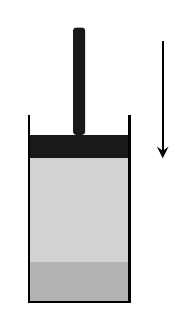
\begin{tikzpicture}[>=stealth,scale=0.85]
\fill[gray!35] (0,0.6) rectangle (1.5,2.15);
\fill[gray!60] (0,0) rectangle (1.5,0.6);
\fill[black!90] (0,2.15) rectangle (1.5,2.5);
\fill[black!90,rounded corners=1pt] (0.66,2.5) rectangle (0.84,4.1);
\draw[line width=0.9pt] (0,2.8)--(0,0)--(1.5,0)--(1.5,2.8);
\draw[->,line width=0.8pt] (2,3.9)--(2,2.15);
\end{tikzpicture}
\end{center}
В цилиндре под поршнем находятся жидкость и её насыщенный пар (см. рисунок). Как изменятся давление и концентрация молекул пара при медленном перемещении поршня вниз, если температура останется неизменной? В процессе движения поршень не касается поверхности жидкости.

Для каждой величины определите соответствующий характер изменения:
\begin{enumerate}
\item увеличится
\item уменьшится
\item не изменится
\end{enumerate}
\TaskChangeTable{Давление пара}{Концентрация молекул пара}
}{
\smallskip\noindent\textbf{Решение от GPT}\par
При медленном изотермическом сжатии часть насыщенного пара конденсируется. Пока присутствуют жидкость и пар, давление \(p_{\text{нас}}(T)\) при неизменной температуре постоянно (\(3\)). Из \(n=p_{\text{нас}}/(kT)\) следует, что концентрация молекул пара также не изменяется (\(3\)).

Ответ: \(33\).
}

% Source 6209: https://phys-ege.sdamgia.ru/problem?id=6209
\BankTask{6209}{
В закрытом сосуде находится $2\,\text{г}$ водяного пара под давлением $50$ кПа и при температуре $100$ ºС. Не изменяя температуры, объем сосуда уменьшили в $4$ раза. Найдите массу образовавшейся при этом воды. Ответ приведите в граммах.
}{
\smallskip\noindent\textbf{Решение}\par
При уменьшении объема сосуда будет увеличиваться давление газа. Достигнув давления насыщенного пара давление перестанет меняться. При дальнейшем уменьшении объема сосуда давление перестанет меняться, но из газа начнет конденсироваться жидкость. Вспомним, что вода кипит при температуре $100$ \ensuremath{{}^\circ}C и нормальном давлении $10^{5}$ Па. Следовательно, давление насыщенного пара при температуре $100$ \ensuremath{{}^\circ}C для воды составляет $100$ кПа. Напишем уравнение Клапейрона  — Менделеева для первого и второго состояний газа.

\[p_1V_1= \frac{m_1}{\mu} RT,p_2V_2= \frac{m_2}{\mu} RT,\]

где $m_1$  — масса газа в первом состоянии, $m_2$  — масса газа во втором состоянии. Из этих соотношений находим массу газа во втором состоянии:

\[m_2= \frac{p_2V_2}{p_1V_1} m_1= \frac{p_2V_2}{p_1 \cdot 4V_2} = \frac{100}{50 \cdot 4} \cdot 2=1\,\text{г}.\]

Масса пара во втором состоянии равна $1\,\text{г}$, следовательно, масса образовавшейся воды $2$ − $1$  =  $1\,\text{г}$.

Ответ: $1\,\text{г}$.
}

% Source 42650: https://phys-ege.sdamgia.ru/problem?id=42650
\BankTask{42650}{
\begin{center}\begin{tikzpicture}[task graph,>=stealth]\draw[gray!65,xstep=.28,ystep=.29](0,0)grid(5.6,4.64);
\draw[->](0,0)--(6.8,0)node[below]{\(t,\,^\circ\text{C}\)};
\draw[->](0,0)--(0,5.2)node[left]{\(p_{\text{н}},\,\text{гПа}\)};
\node[below left]at(0,0){\(0\)};
\foreach \x/\label in {1.4/10,2.8/20,4.2/30,5.6/40}{\node[below]at(\x,0){\(\label\)};}
\foreach \y/\label in {1.16/20,2.32/40,3.48/60,4.64/80}{\node[left]at(0,\y){\(\label\)};}
\draw[smooth] plot coordinates{(0,.47)(.7,.66)(1.4,.83)(2.24,1.16)(2.8,1.53)(3.5,2.1)(4.2,2.78)(4.9,3.65)(5.53,4.99)};\end{tikzpicture}\end{center}
В сосуде ёмкостью V  =  $2$ л, воздух из которого был откачан до высокого вакуума, разбили заполненную водой ампулу ёмкостью $V_{1}$  =  $4\,\text{см}^{3}$. Какая часть воды, содержавшейся в ампуле, испарилась? В сосуде поддерживалась температура $16 ^\circ\text{C}.$ Зависимость давления насыщенного пара от температуры представлена на графике. Объёмом воды в сосуде можно пренебречь.
}{
\smallskip\noindent\textbf{Решение}\par
После того, как в сосуде разбили пробирку, в нем оказалась вода массой $m_{\,\text{в}}=\rho V_{\,\text{п}}=10 ^3 \cdot 4 \cdot 10 ^{ - 6 } =4\,\text{г}.$ Поскольку в сосуде находится высокий вакуум, то при температуре $16$ \ensuremath{{}^\circ}C вода закипит и превратится в пар. Если пар в сосуде стал насыщенным, то, согласно графику, его давление должно быть равным $20$ гПа.
При температуре $16$ \ensuremath{{}^\circ}C ($289$ К) сосуде в результате испарения воды оказался пар, массу  которого найдем из уравнения Менделеева-Клапейрона $pV= \frac{m}{M} RT$ при условии, если бы пар стал насыщенным:

\[m= \frac{pVM}{RT} = \frac{2 \cdot 10 ^3 \cdot 2 \cdot 10 ^{ - 3 } \cdot 18 \cdot 10 ^{ - 3 }}{8{,}31 \cdot 289} \approx 30 \cdot 10 ^{ - 3 } \,\text{г}.\]

Отсюда делаем вывод, что пар стал насыщенным, а из пробирки испарилась часть воды, равная

\[\frac{m}{m_{\,\text{в}}} = \frac{30 \cdot 10 ^{ - 3 }}{4} =0{,}0075.\]

Ответ: $0{,}0075$.
}

% Source 6281: https://phys-ege.sdamgia.ru/problem?id=6281
\BankTask{6281}{
В сосуде под поршнем при температуре $100$ ºС находится $2\,\text{г}$ водяного пара и такое же количество воды. Не изменяя температуры, объем сосуда увеличили в $3$ раза. Определите массу воды, перешедшей при этом в пар. Ответ приведите в граммах.
}{
\smallskip\noindent\textbf{Решение}\par
Под поршнем находится насыщенный пар, то есть жидкость и газ находятся в динамическом равновесии друг с другом. При каждом небольшом увеличении объема сосуда давление газа немного уменьшается. В результате этого часть молекул воды переходит из жидкого состояния в газообразное, динамическое равновесие восстанавливается. Поэтому, пока вся вода не перейдет в газообразное состояние, давление пара над жидкостью не будет меняться. Вспомним, что вода кипит при температуре $100$ °C и нормальном давлении $10^{5}$ Па. Следовательно, давление насыщенного пара при температуре $100$ °C для воды составляет $100$ кПа. Напишем уравнение Клапейрона  — Менделеева для первого и второго состояний газа.

\[p_1V_1= \frac{m_1}{\mu} RT,p_2V_2= \frac{m_2}{\mu} RT,\]

где $m_1$  — масса газа в первом состоянии, $m_2$  — масса газа во втором состоянии. Из этих соотношений находим массу газа во втором состоянии:

\[m_2= \frac{p_2V_2}{p_1V_1} m_1= \frac{p_1 \cdot 3V_1}{p_1V_1} m_1= \frac{3}{1} \cdot 2=6\,\text{г}.\]

В результате расчетов получается, что в газообразное состояние должны были бы перейти $6\,\text{г} - 2\,\text{г}=4\,\text{г}$ воды. Учитывая, что воды в жидком состоянии лишь $2\,\text{г}$, получаем что вся вода перейдет в газообразное состояние, то есть масса воды, перешедшей в пар, равна $2\,\text{г}$.

Ответ: $2\,\text{г}$.
}

% Source 3721: https://phys-ege.sdamgia.ru/problem?id=3721
\BankTask{3721}{
В закрытом сосуде под поршнем находится $4\,\text{г}$ насыщенного водяного пара. Двигая поршень, занимаемый паром объем уменьшили в $2$ раза, поддерживая температуру сосуда и его содержимого постоянной и равной $100$ °C. Какое количество теплоты было при этом отведено от сосуда?
}{
\smallskip\noindent\textbf{Решение}\par
Насыщенный пар  — это пар, имеющий максимально возможную концентрацию при данной температуре, при этом концентрация пара зависит только от температуры. Поскольку при уменьшении объема в два раза, температуру сосуда и его содержимого поддерживали постоянной, заключаем, что концентрация насыщенного пара не изменялась, а значит, в результате такого сжатия сконденсировалась ровно половина всего пара, то есть $2\,\text{г}$.
По первому началу термодинамики изменение внутренней энергии системы равно разности работы, совершаемой над системой, и количеством теплоты, забираемой у системы:

$\Delta U=A - Q ,$ откуда $Q= - \Delta U + A.$

При конденсировании $2\,\text{г}$ пара его внутренняя энергия уменьшается:

\[\Delta U= - L\Delta m= - 2{,}3 \cdot 10 ^{6} \,\text{Дж/кг} \cdot 0{,}002 \,\text{кг}= - 4600\,\text{Дж}.\]

При сжатии над паром совершается работа:

\[A=p\Delta V= \frac{pV_0}{2} = \frac{m}{2M} RT= \frac{4\,\text{г}}{2 \cdot 18\,\text{г/моль}} \cdot 8{,}31\,\text{Дж}/ ( \,\text{моль} \cdot \,\text{К} ) \cdot 373\,\text{К}\approx344\,\text{Дж}.\]

Количество забираемой теплоты равно:

\[Q=4600\,\text{Дж} + 344\,\text{Дж}\approx5\,\text{кДж}.\]

Ответ: $5\,\text{кДж}$.
}

% Source 38662: https://phys-ege.sdamgia.ru/problem?id=38662
\BankTask{38662}{
Вертикальный цилиндрический сосуд с влажным воздухом влажностью $\varphi$ закрыт невесомым поршнем площадью S, способным скользить без трения. В начальном состоянии поршень находится в равновесии. На поршень медленно насыпают песок. Определите минимальную массу песка m, при которой на стенках сосуда появится роса. Температура в сосуде поддерживается постоянной. Внешнее атмосферное давление равняется $p_{0}$.
}{
\smallskip\noindent\textbf{Решение}\par
В первом состоянии поршень невесомый, поэтому давление влажного воздуха равно атмосферному давлению $p_1=p_0.$ Из формулы влажности $\varphi = \frac{p_{\,\text{п}1}}{p_{\,\text{нп}}} ,$ где $p_{\,\text{п}1}$  — парциальное давление водяного пара в первом состоянии, $p_{\,\text{нп}}$  — давление насыщенного пара при данной температуре.
Во втором состоянии выпала роса, что означает  — пар стал насыщенным. Следовательно,  в сосуде давление водяных паров $p_{\,\text{п}2}$ стало равным $p_{\,\text{нп}}$. 
Поршень в равновесии, следовательно, $p_2 = p_0 + \frac{mg}{S} ,$  где $p_{2}$  — давление пара после насыпания песка.
И для ненасыщенного водяного пара, и для влажного воздуха можно применить закон Бойля-Мариотта при изотермическом процессе:

$\frac{V_2}{V_1} = \frac{p_1}{p_2}$
$\frac{V_2}{V_1} = \frac{p_{\,\text{п}1}}{p_{\,\text{п}2}} ,$

где $V_{1}$ и $V_{2}$ начальный и конечные объемы влажного воздуха в сосуде под поршнем. Из этих соотношений получаем:

\[\frac{p_1}{p_2} = \frac{p_{\,\text{п}1}}{p_{\,\text{п}2}} .\]

 Объединяя эти уравнения, получаем, что масса песка равна

\[m= \frac{p_0S ( 1 - \varphi )}{\varphi g} .\]

Ответ: $m = \frac{p_0 S}{g} \cdot ( \frac{1 - \varphi}{\varphi} ) .$
}

\end{document}
